\begin{tutorial}{Нить ДНК}

Задача на первый взгляд является пространственной, но ее очень легко перевести на плоскость. Для этого разрежем цилиндр параллельно оси $OO^\prime$ и развернем его, тогда цилиндр превращается в прямоугольник. Так как точка $M$ вращается вокруг оси $OO^\prime$ равномерно и движется вверх тоже равномерно, то на плоскости прямоугольника винтовая линия будет представлена множеством параллельных отрезков, суммарную длину которых и требуется найти. 

\begin{center}
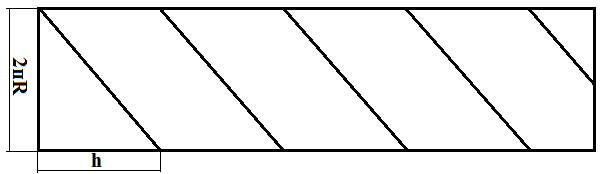
\includegraphics[scale=0.4]{expansion.png}
\end{center}

Длину одного отрезка легко найти, используя теорему Пифагора: 

$$L_1=\sqrt{4\pi^2 R^2 + h^2.}$$

Тогда длина одного витка ДНК может быть вычислена следующим образом:

$$L_{DNA} = L_1 \frac{L}{h}.$$

\end{tutorial}
